\documentclass[12pt,a4paper]{article}
\usepackage[utf8]{inputenc}
\usepackage[spanish]{babel}
\usepackage{geometry}
\usepackage[
    backend=biber,
    style=numeric,
    sorting=ynt
]{biblatex}
\usepackage{csquotes}
\usepackage{siunitx}
\usepackage{physics}
\usepackage{lmodern}
\usepackage{graphicx}
\usepackage{float}
\usepackage{algorithm}
\usepackage{algpseudocode}
\usepackage{listings}
\lstdefinestyle{codestyle}{
  basicstyle=\ttfamily\footnotesize,
  columns=fullflexible,
  keepspaces=true,
  numbers=left,
  frame=single,
  tabsize=4,
  breaklines=true,
  breakatwhitespace=true,
  captionpos=b
}
\lstdefinelanguage{ts}{
  keywords={typeof, new, true, false, catch, function, return, null, catch, switch, var, if, in, while, do, else, case, break, private, readonly, let, for, const, of},
  keywordstyle=\ttfamily\bfseries,
}
\lstset{style=codestyle}


\addbibresource{refs.bib}
\geometry{a4paper, margin=2.5cm}

\begin{document}

\begin{titlepage}
    \centering
    \vspace*{1.5cm}
    
    {\scshape\LARGE Universidad Nacional de Tres de Febrero \par}
    \vspace{0.5cm}
    {\large Ingeniería en Computación \par}
    
    \vspace{2.5cm}
    
    {\huge \textbf{Física II} \par}
    \vspace{0.5cm}
    {\Large Plan 2022\par}
    
    \vspace{2cm}
    {\Large Trabajo Práctico Final \par}
    {\Large Simulador de ley de Biot-Savart \par}
    \vspace{0.5cm}
    {\large Julio 2026\par}
    
    \vspace{3.5cm}
    
    \begin{minipage}{0.45\textwidth}
        \begin{flushleft} \large
            \emph{Autor:}\\
            Juan Cruz Dal Bello
        \end{flushleft}
    \end{minipage}
    \hfill
    \begin{minipage}{0.45\textwidth}
        \begin{flushright} \large
            \emph{Docentes:} \\
            Dr. Juan Carlos Muñoz \\
            Dr. Pablo Germán König
        \end{flushright}
    \end{minipage}
    
    \vfill
\end{titlepage}

\clearpage

\tableofcontents

\newpage

\section{Introducción y objetivos}
El trabajo presentado es un simulador 2D interactivo que ilustra el comportamiento del campo magnético alrededor de un conductor de forma y longitud arbitrarios por el que pasa una corriente uniforme.

A diferencia de los conductores de forma simétrica (ej: circunferencias, líneas rectas), de los que se puede extraer una ecuación para sus casos particulares para simplificar las operaciones, cada conductor de forma arbitraria requiere hacer cálculos a lo largo de toda su longitud para obtener resultados exactos. Esta necesidad dificulta visualizar el comportamiento de factores físicos que ocurren en su cercanía.

Un simulador que permita explorar estos casos que se alejan de las formas idealizadas sería una gran ayuda didáctica, permitiría explorar su respuesta de forma más sencilla, y reduciría el margen de error debido a la gran cantidad de cálculos manuales que requieren cambios muy sutiles en los valores usados.

\section{Fundamento físico}
\subsection{Ley de Biot-Savart}
El funcionamiento físico del simulador se basa en la ley de Biot-Savart \cite{serway}, que permite averiguar el valor del campo magnético $d\va{B}$ en algún punto $P$ del espacio asociado a un elemento de longitud $d \va{l}$ por el que pasa una corriente $I$ mediante la ecuación

\begin{equation} \label{eq:biot_savart}
    d\va{B} = \frac{\mu_0}{4 \pi} \frac{I d \va{l} \times \vu{r}}{r^2}
\end{equation}

donde $\mu_0$ es la permeabilidad del espacio libre:

\begin{equation}
    \mu_0 =  4\pi \times 10^{-7} \ \mathrm{T \cdot m / A}
\end{equation}

y con $\vu{r}$ siendo un vector unitario desde $d \va{l}$ hasta $P$, y $r$ la distancia entre ambos. Los cálculos se hicieron teniendo en cuenta una corriente de intensidad constante a lo largo de todo el conductor.

Para obtener el campo magnético $\va{B}$ en cada punto es necesario sumar la contribución de todos los elementos $d\va{l}$ a lo largo del conductor, integrando la ecuación (\ref{eq:biot_savart}):

\begin{equation}
    \va{B} = \frac{\mu_0 I}{4 \pi} \int \frac{d \va{l} \times \vu{r}}{r^2}
\end{equation}

\subsection{Implementación y limitaciones de la simulación}
\subsubsection{Espacio de la simulación}
A modo de delimitar el espacio y establecer una visualización estandarizada independientemente del dispositivo en el que se muestre, se usó un display de $800 \times 600 \ \si{px}$ para el trazado del conductor, y se estableció que $1 \ \si{px}$ de la representación se corresponde con $1$cm ($1 \ \si{px} \ \widehat{=} \ 1 \ \si{cm}$).

Al trabajar con un trazo únicamente en el plano $XY$, la representación de los vectores del campo magnético se representa con ($\times$) para indicar un vector saliendo de la pantalla, y con ($\cdot$) para uno entrando a la pantalla.

\subsubsection{Discretización y suma de Riemann}
El mayor problema para implementar la ecuación mencionada es que está pensada para una integral, sobre infinitos valores, que no puede calcularse de forma analítica en el software. Para resolver esto, se usó como base el concepto de la suma de Riemann \cite{stewart}:
\begin{equation}
    \int_{a}^{b} f(x) dx = \lim_{n \to \infty} \sum_{i=1}^n f(x_i) \Delta x_i
\end{equation}

que propone que se puede aproximar a la integral por medio de una sumatoria de términos finitos, con una precisión proporcional a la cantidad de puntos de muestra $x_i$. En la simulación, estos términos están relacionados a las partes del conductor dibujado por el usuario, conformadas por los segmentos que conectan cada punto del trazo, de manera que a mayor cantidad de segmentos disponibles aumenta la exactitud de los cálculos:

\begin{equation}\label{eq:aproximacion_campo_magnetico}
    \va{B} \approx \frac{\mu_0 I}{4 \pi} \sum_{i=1}^{n} \frac{\Delta \va{l}_i \times \vu{r}_i}{r^{2}_{i}}
\end{equation}

\subsubsection{Puntos de singularidad}
La intensidad del campo magnético en un punto $P$ es inversamente proporcional al cuadrado de la distancia con respecto al conductor ($\vb{B} \propto \frac{1}{r^2}$), por lo que su magnitud aumenta conforme esa distancia se acorta. Cuando $r \to 0$, matemáticamente se corresponde que $\vb{B} \to \infty$.

Se usó un valor arbitrario \verb|SINGULARITY_THRESHOLD = 0.05| que representa 0.05 \si{cm} en el espacio de la simulación.
Cuando se dan estos casos en el simulador, en lugar de mostrar la magnitud se aclara que $r \to 0$, como un caso particular.

\subsubsection{Intensidad de la corriente}
Para que la intensidad de la corriente fuese un parámetro controlado por el usuario y que no requiriese cálculos innecesarios, se aplicó como un multiplicador luego del cálculo de $\va{B}$, por lo que la implementación de la ecuación (\ref{eq:aproximacion_campo_magnetico}) se realiza con $I=1$.

\subsubsection{Algoritmo}
Teniendo claras las limitaciones del pasaje de la teoría pura a la computadora, se procedió a pensar el algoritmo discreto con los segmentos $\Delta\va{l}$ del conductor que se obtienen de la interacción del usuario con la interfaz:

\begin{algorithm}[H]
\caption{Estimación del campo magnético en un punto $P$}
\label{alg:biot_savart}
\begin{algorithmic}[1]
\Procedure{CalcularCampoMagneticoEn}{$\vb{P}, \text{conductor}$}
    \State $\va{B} \gets (0, 0, 0)$
    \State $\text{UMBRAL\_SINGULARIDAD} \gets 0.05$
    
    \For{\textbf{each} $\Delta\va{l}$ \textbf{in} $conductor$}
        \State $\va{r} \gets \vb{P} - \Delta\va{l}$
        
        \If{$\vb{r} < \text{UMBRAL\_SINGULARIDAD}$}  \Comment{Caso particular}
            \State \Return \textbf{nulo}
        \EndIf 
        
        \State $\vu{r} \gets \frac{\va{r}}{\vb{r}}$
        
        \State $\va{B} \gets \va{B} + \frac{\Delta\va{l} \times \vu{r}}{\vb{r^2}}$ \Comment{Suma de Riemann}
    \EndFor
    
    \State $\va{B} \gets \va{B} \cdot \frac{\mu_0}{4 \pi}$
    
    \State \Return $\va{B}$
\EndProcedure
\end{algorithmic}
\end{algorithm}

\subsubsection{Implementación del algoritmo}

Una vez representados los vectores tridimensionales ($\va{V}=(x,y,z)$) y las operaciones relacionadas, se procedió a pasar el algoritmo al código:

\lstinputlisting[
    language=ts,
    caption={Implementación del algoritmo con la ley de Biot-Savart en TypeScript},
    label={listing_biot_savart}
]{code/biot_savart.ts}

\subsubsection{Stack tecnológico}
El simulador está desarrollado en TypeScript para la parte lógica, junto con HTML y CSS para la visualización, y Vite para el manejo y organización del proyecto. Puede ejecutarse de manera local o probarse de manera online (\url{https://jcdalbello.github.io/fisica_2_tp_final_simulacion/}) en cualquier dispositivo.

\section{Interfaz y uso del simulador}
La interfaz del simulador está compuesta por el slider de intensidad de la corriente ($I \in [1;100]$), los botones para invertir el sentido de la corriente y limpiar los trazos, el indicador de intensidad del campo magnético en $\si{\mu T}$, y el canvas sobre el que se dibuja el conductor:

\begin{figure}[H]
    \centering
    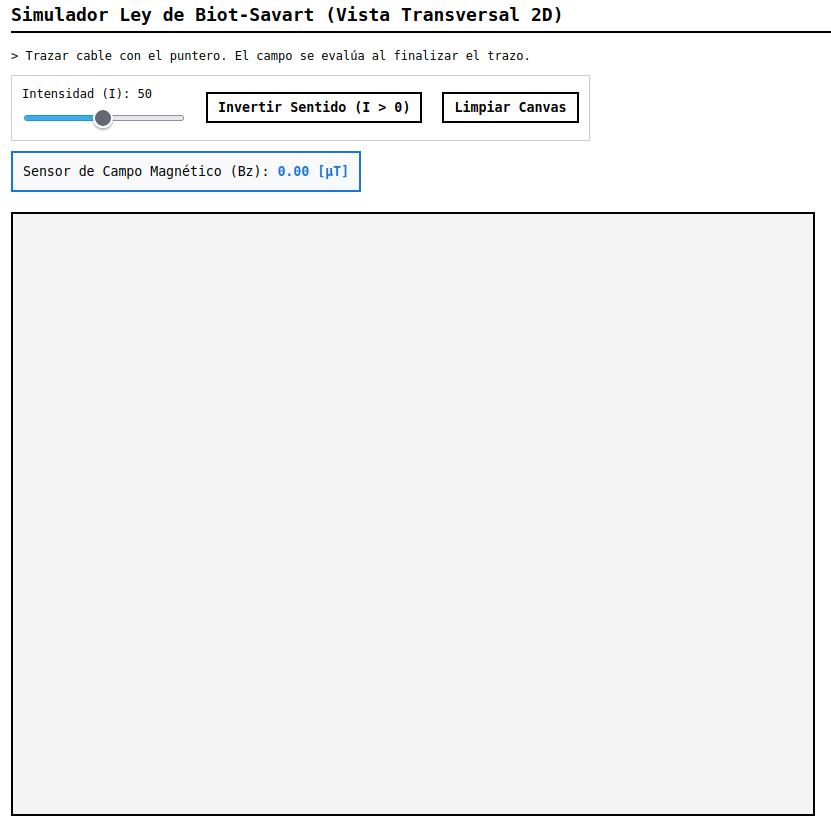
\includegraphics[width=\textwidth]{imagenes/interfaz_vacia.png}
    \caption{Interfaz vacía}
    \label{fig:interfaz_vacia}
\end{figure}

\clearpage

Para dibujar un conductor en el canvas, se debe hacer click y mantenerlo presionado sobre su superficie, arrastrar el mouse para dibujar, y soltar cuando se quiera terminar el trazo:

\begin{figure}[H]
    \centering
    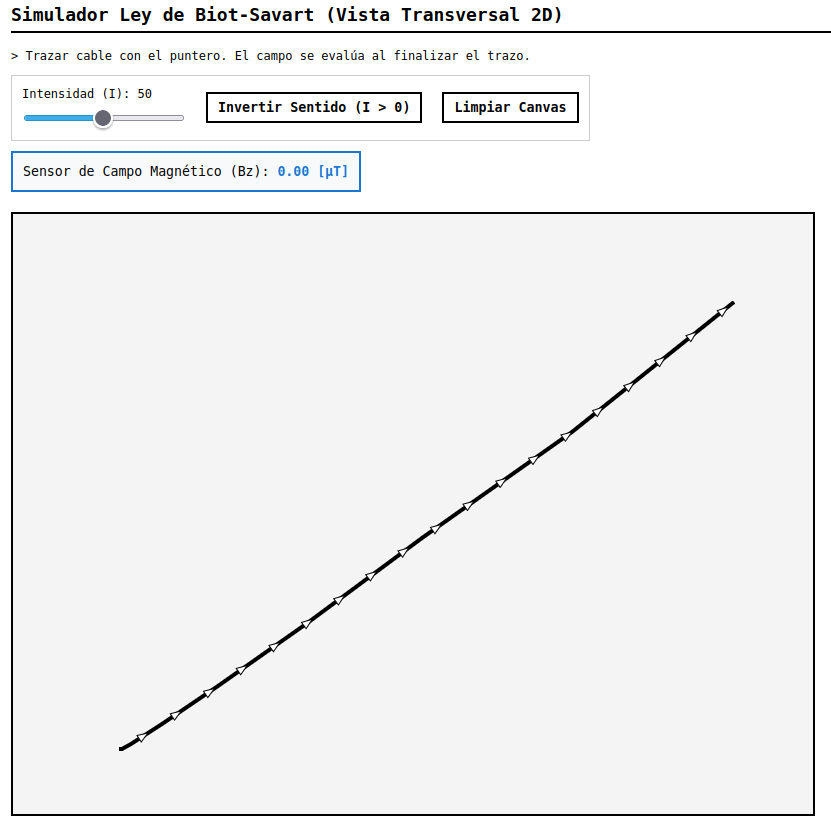
\includegraphics[width=\textwidth]{imagenes/trazo.png}
    \caption{Trazo con el mouse}
    \label{fig:trazo}
\end{figure}

\clearpage

Una vez dibujado el conductor, el simulador va a mostrar los símbolos correspondientes al campo magnético en los puntos cercanos al conductor:

\begin{figure}[H]
    \centering
    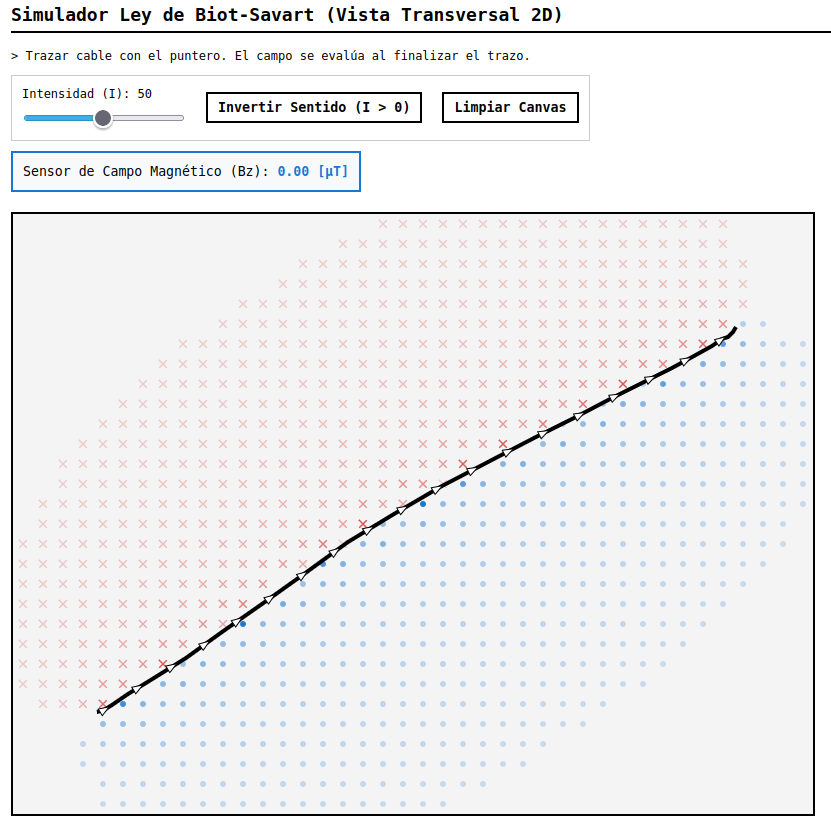
\includegraphics[width=\textwidth]{imagenes/campos_magneticos.png}
    \caption{Campos magnéticos cerca del conductor}
    \label{fig:campos_mageneticos}
\end{figure}

\clearpage

Las flechas a lo largo del conductor indican el sentido de la corriente, y su velocidad da un indicativo de su intensidad. Usando el botón correspondiente se puede invertir el sentido de la corriente y actualizar los campos magnéticos:

\begin{figure}[H]
    \centering
    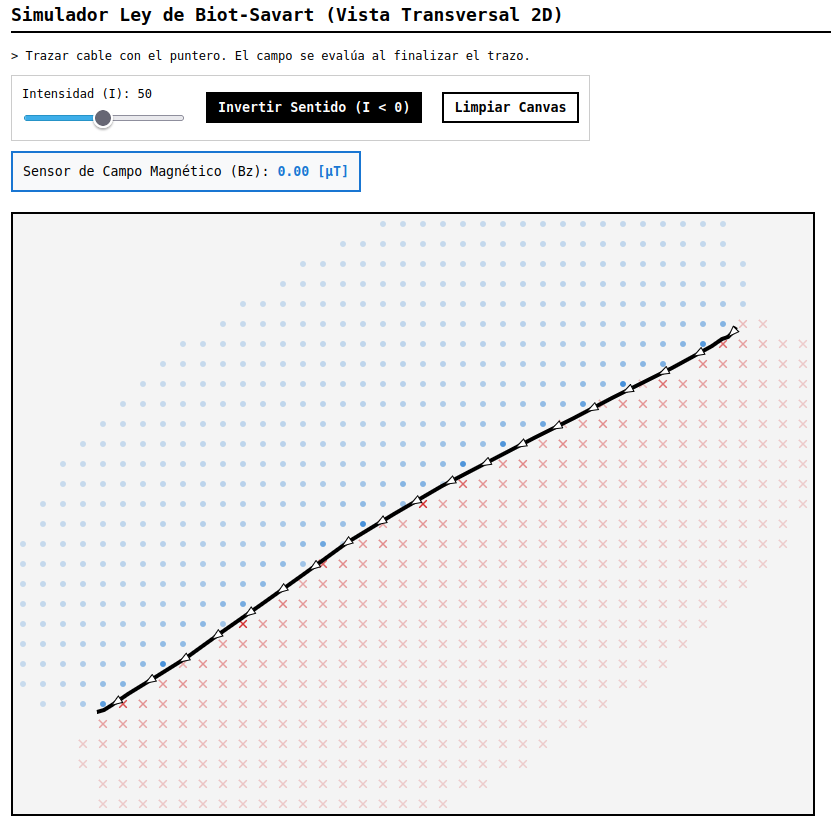
\includegraphics[width=\textwidth]{imagenes/invertir_corriente.png}
    \caption{Invertir el sentido de la corriente}
    \label{fig:invertir_corriente}
\end{figure}

\clearpage

Una vez renderizados los símbolos de campo magnético, se puede mover el mouse por el canvas para ver la intensidad del campo sobre un punto:

\begin{figure}[H]
    \centering
    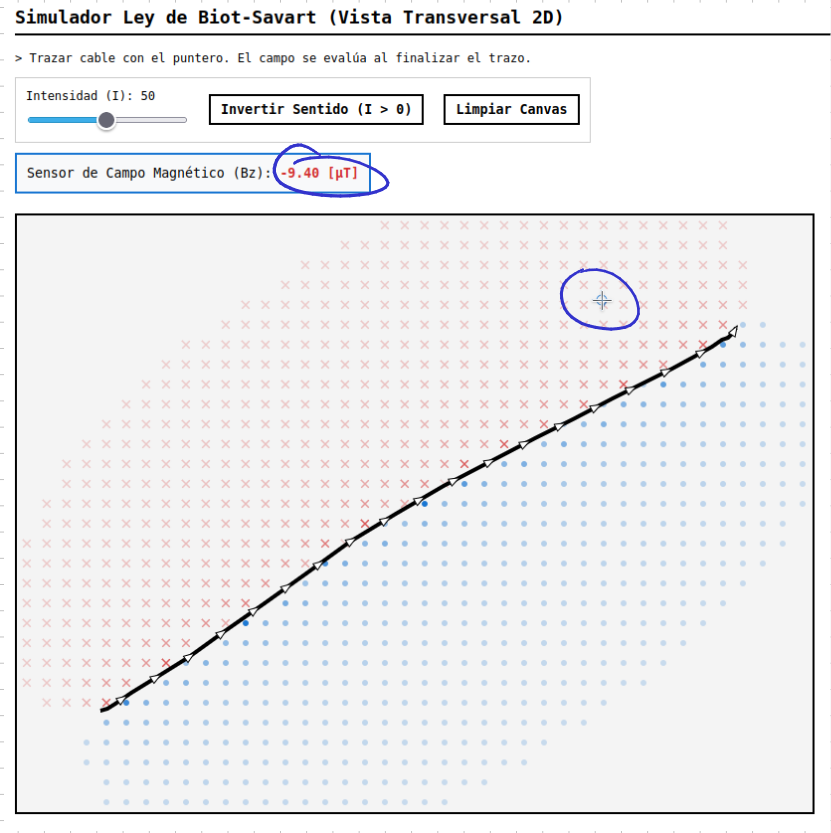
\includegraphics[width=\textwidth]{imagenes/sensor.png}
    \caption{Sensor de corriente sobre el canvas}
    \label{fig:sensor}
\end{figure}

\section{Conclusión}
El simulador presentado es una aproximación numérica por segmentos al análisis de campos magnéticos con respecto a geometrías no regulares en un plano XY que afectan a un espacio 3D. Esta limitación restringe la veracidad de los resultados a un ámbito meramente didáctico.
A pesar de las limitaciones, permite visualizar un contenido que de otra manera sería difícil poder observar en la práctica, facilitando la comprobación de fundamentos teóricos.
% ---------------------------------------------------------------------------

\clearpage

\section*{Disponibilidad de código}
El simulador puede probarse de manera online en \url{https://jcdalbello.github.io/fisica_2_tp_final_simulacion/}.

Todo el material relacionado al proyecto, que incluye tanto el simulador como el presente documento y el código \LaTeX{} usado para generarlo, se encuentran disponibles en \url{https://github.com/jcdalbello/fisica_2_tp_final_simulacion}.

\printbibliography

\end{document}